\documentclass[a4paper]{article}

% Packages
\usepackage{graphicx}
\usepackage[margin=1in]{geometry}
\usepackage[backend=bibtex]{biblatex}
\usepackage{comment}
\usepackage{hyperref}


\addbibresource{references.bib}

\title{Evaluation of Pre-Trained Models for Translation in Different Languages}
\author{Stefan Liemawan Adji}
\date{\today}

\begin{document}

\maketitle

\section{Introduction}

According to Ethnologue \cite{ethnologue-2024}, 7,164 languages currently exist and in use today, with 40\% of them considered endangered. As of July 2024, 243 languages are supported by Google Translate (according to Wikipedia \cite{wikipedia-google-translate}). In modern times, the need for translation services has surged due to the growing exchange of information across different regions that speak various languages \cite{okpor-2014-machine-ta}.

Machine translation (MT) is the task of automatically translating from one language to another. This can be done through text or audio. It can be traced back to 1949 \cite{weaver-1999}, with the first public demonstration of an MT system on January 7, 1954, in collaboration with IBM, where 49 Russian sentences were translated into English using a limited vocabulary of 250 words and 6 grammar rules \cite{hutchins-2006-first-mt}. However, over the next several decades, growth were limited for machine translation, with 1956-1966 considered the decade of high expectation and disillusion, and 1967-1976 dubbed 'the quiet decade' \cite{hutchins-2001-mt-50-years}. Then in 1989, the dominance of the rule-based approach has been challenged by the rise of new methods and strategies, collectively referred to as ‘corpus-based’ methods (data-driven) \cite{hutchins-1994-research-methods-mt,hutchins-1998-development-mt}. Subsequently, statistics-based approaches for MT re-emerged, bolstered by the recent success of probabilistic techniques in speech recognition. Statistical machine translation \cite{lopez-2008-smt} dominated the domain between late 1990s through the early 2010s, before largely being surpassed by neural machine translation (NMT) \cite{cho-2014-properties,sutskever-2014-seq2seq}. Finally, since the introduction of Transformers in 2017 \cite{vaswani-2017-attention}, Natural Language Processing (NLP) and machine translation in particular reached a giant milestone. The following years saw the birth of Large Language Models (LLMs) such as BERT \cite{devlin-2019-bert}, GPT \cite{openai-2024-gpt4}, and T5 \cite{raffel-2023-t5}, which revolutionised both MT and the whole field of NLP. Soon after, several pre-trained models that are specifically designed for machine translation emerged, namely mBART \cite{liu-2020-mbart}, mT5 \cite{xue-2021-mt5}, and NLLB \cite{nllb200}.

Since LLMs require vast amounts of training data, the availability of parallel corpora is crucial for building effective models. The lack of extensive parallel corpora, especially for low-resource languages, leads to suboptimal performance in NMT techniques compared to their high-resource counterparts \cite{ranathunga-2023-nmt-low-res}.


OPUS \cite{opus} is a comprehensive collection of open-source parallel corpora used extensively in the field of machine translation (MT). It includes corpora for 744 languages and contains over 1,210 different datasets, amassing a total of 45,945,946,108 sentence pairs. Tatoeba \cite{tatoeba} is another prominent resource in the field of MT and NLP, known for its extensive collection of translated sentences. As of July 2024, it contains 12,186,207 sentences over 423 supported languages, growing daily through volunteer contributions.

pre-trained models...


Through simple experimentation and analysis, this paper aims to evaluate existing pre-trained models across different languages
and contribute valuable insights into the current state of machine translation technology.

\section{Literature Review}

\subsection{Neural Machine Translation (NMT)}

The encoder-decoder approach \cite{cho-2014-properties} remains as the foundation architecture for many sequence-to-sequence models in natural language processing, especially machine translation.


\subsection{One-to-one Models}

One-to-One Translation refers to a translation approach where a model is specifically trained to translate between one source language and one target language. This setup is characterised by having a dedicated model for each unique language pair.

The OPUS-MT by Helsinki-NLP \cite{tiedemann-2020-opus-mt} is a good example of one-to-one translation project, they provide over 1,000 pre-trained translation models for many language pairs, allowing users to perform high-quality translations without needing to train models from scratch.

OpenNMT \cite{klein-etal-2017-opennmt} is another framework that allows for one-to-one translation, although their pre-trained models only support English and German languages.

\subsection{Many-to-many Models}

With the rise of LLMs and pre-trained language models, multilingual machine translation models have received popularity, particularly many-to-many translation.

Multilingual neural machine translation (NMT) allows for the training of a single model capable of translating between multiple source and target languages \cite{aharoni-2019-massively-multilingual}.

Many-to-many translation refers to the capability of a model to translate text between multiple language pairs bidirectionally. This means the model can handle translations from any of the supported source languages to any of the supported target languages, not limited to a single source or target language.

mBart \cite{liu-2020-mbart} (50 languages), NLLB-200 \cite{nllb200} (200 language), PolyLM \cite{wei-2023-polylm} (32 languages), and mt5 \cite{xue-2021-mt5} (101 languages) are some of the most popular many-to-many models.


\subsection{Sequence-to-Sequence Models}

GPT \cite{openai-2024-gpt4}

mBERT \cite{devlin-2019-bert} is the multilingual version of BERT, introduced in the same paper, trained on 104 different languages. However, the model been shown to suffer on low-resource languages \cite{wu-2020-mbert-are-all}.

T5 \cite{raffel-2023-t5} is a Text-to-Text Transfer Transformer model trained on English.

MistralAI \cite{jiang-2023-mistral-7b}


\section{Experiments}

\subsection{Dataset}

Tatoeba is a vast, continuously expanding database consisting sentences and their translations, built through the contributions of thousands of volunteers, offering a tool that allows users to see examples of how words are used in sentences \cite{tatoeba}. They currently have 12,132,349 sentences and 423 supported languages, with around one to two thousand new sentences added daily, on average

Tatoeba is chosen due to its sentence having more daily life sentences...?

To build the dataset,

Sentences in English are downloaded, 1,898,494 sentences (it is unclear why it is less than the number stated in the Tatoeba website). Then for each languages, download sentence pairs compared to English. Merge every language sentences into one big dataframe, only keep where sentences exist for every language

\begin{figure}[htbp]
    \centering
    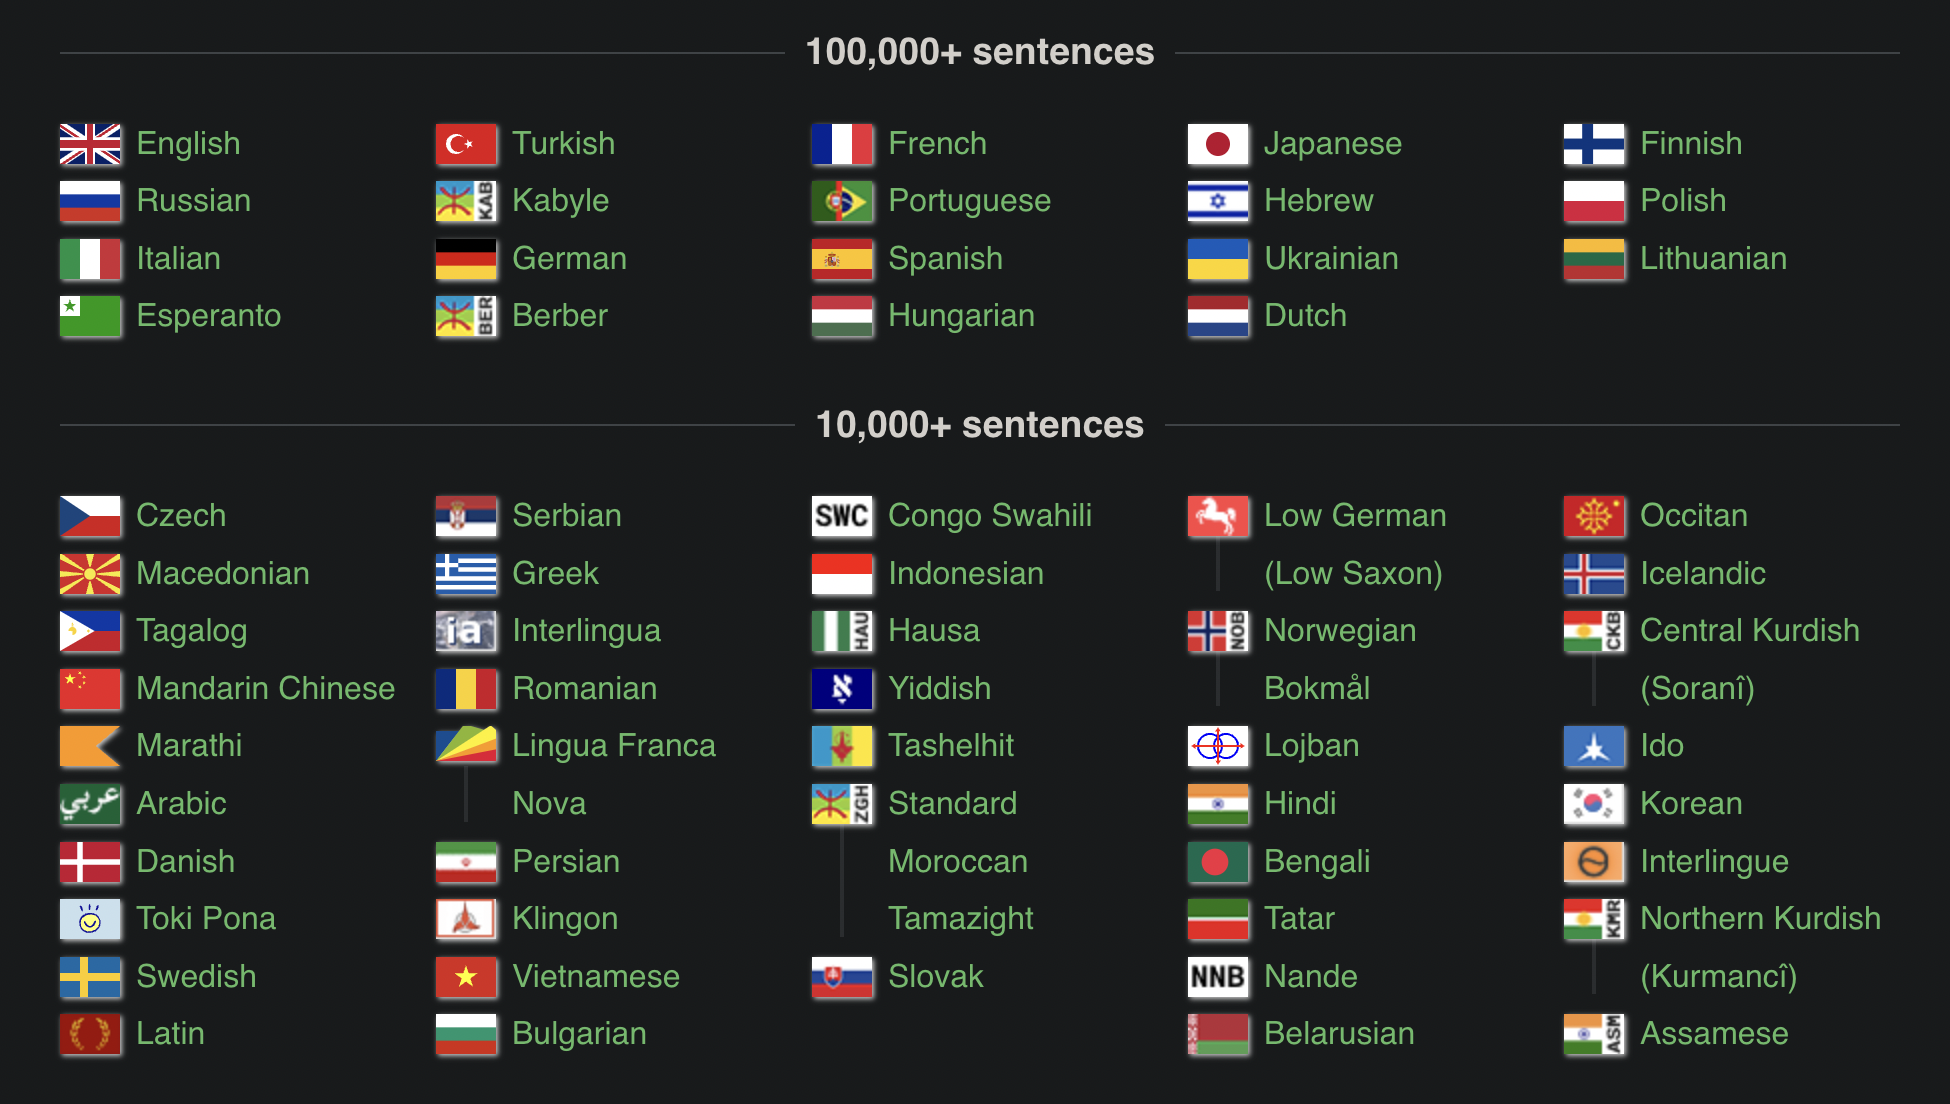
\includegraphics[width=0.9\linewidth]{images/tatoeba_languages.png}
    \caption{Tatoeba languages repository with 10,000+ sentences and 100,000+ sentences \cite{tatoeba}}
    \label{fig:tatoeba_languages}
\end{figure}

Tatoeba English sentence dataset contains 1,905,089 sentences, the largest one in their repository, with Russian in the second place with 1,066,633 sentences. Some of the languages supported in the website is shown in Figure \ref{fig:tatoeba_languages} and Figure \ref{fig:tatoeba_top_bottom_languages}, sorted from the biggest corpus. Low-resource languages such as Rendille, Southern Haida, and Cuyonon can be seen at the bottom of the list, having only a single sentence example. Ancestor languages such as Old Saxon and Old Turkish can also be seen in the list, subsequently with low number of examples.

\begin{figure}[htbp]
    \centering
    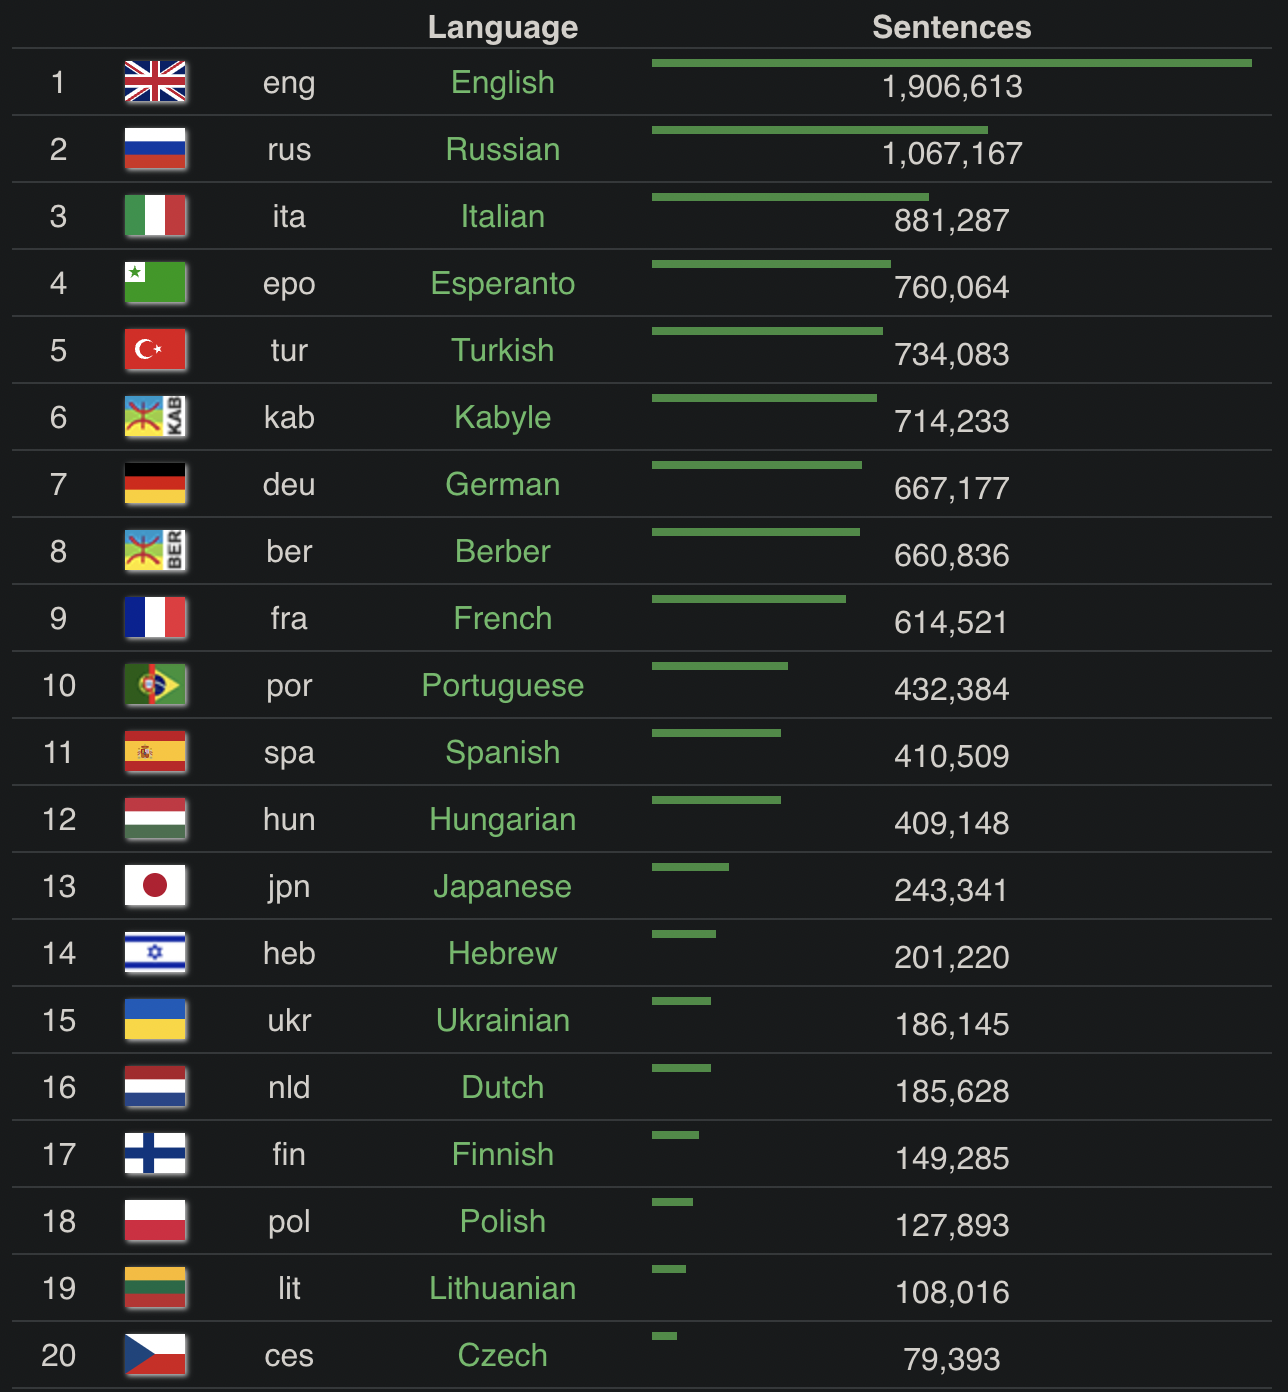
\includegraphics[width=0.5\linewidth]{images/tatoeba_top_20_lang.png}
    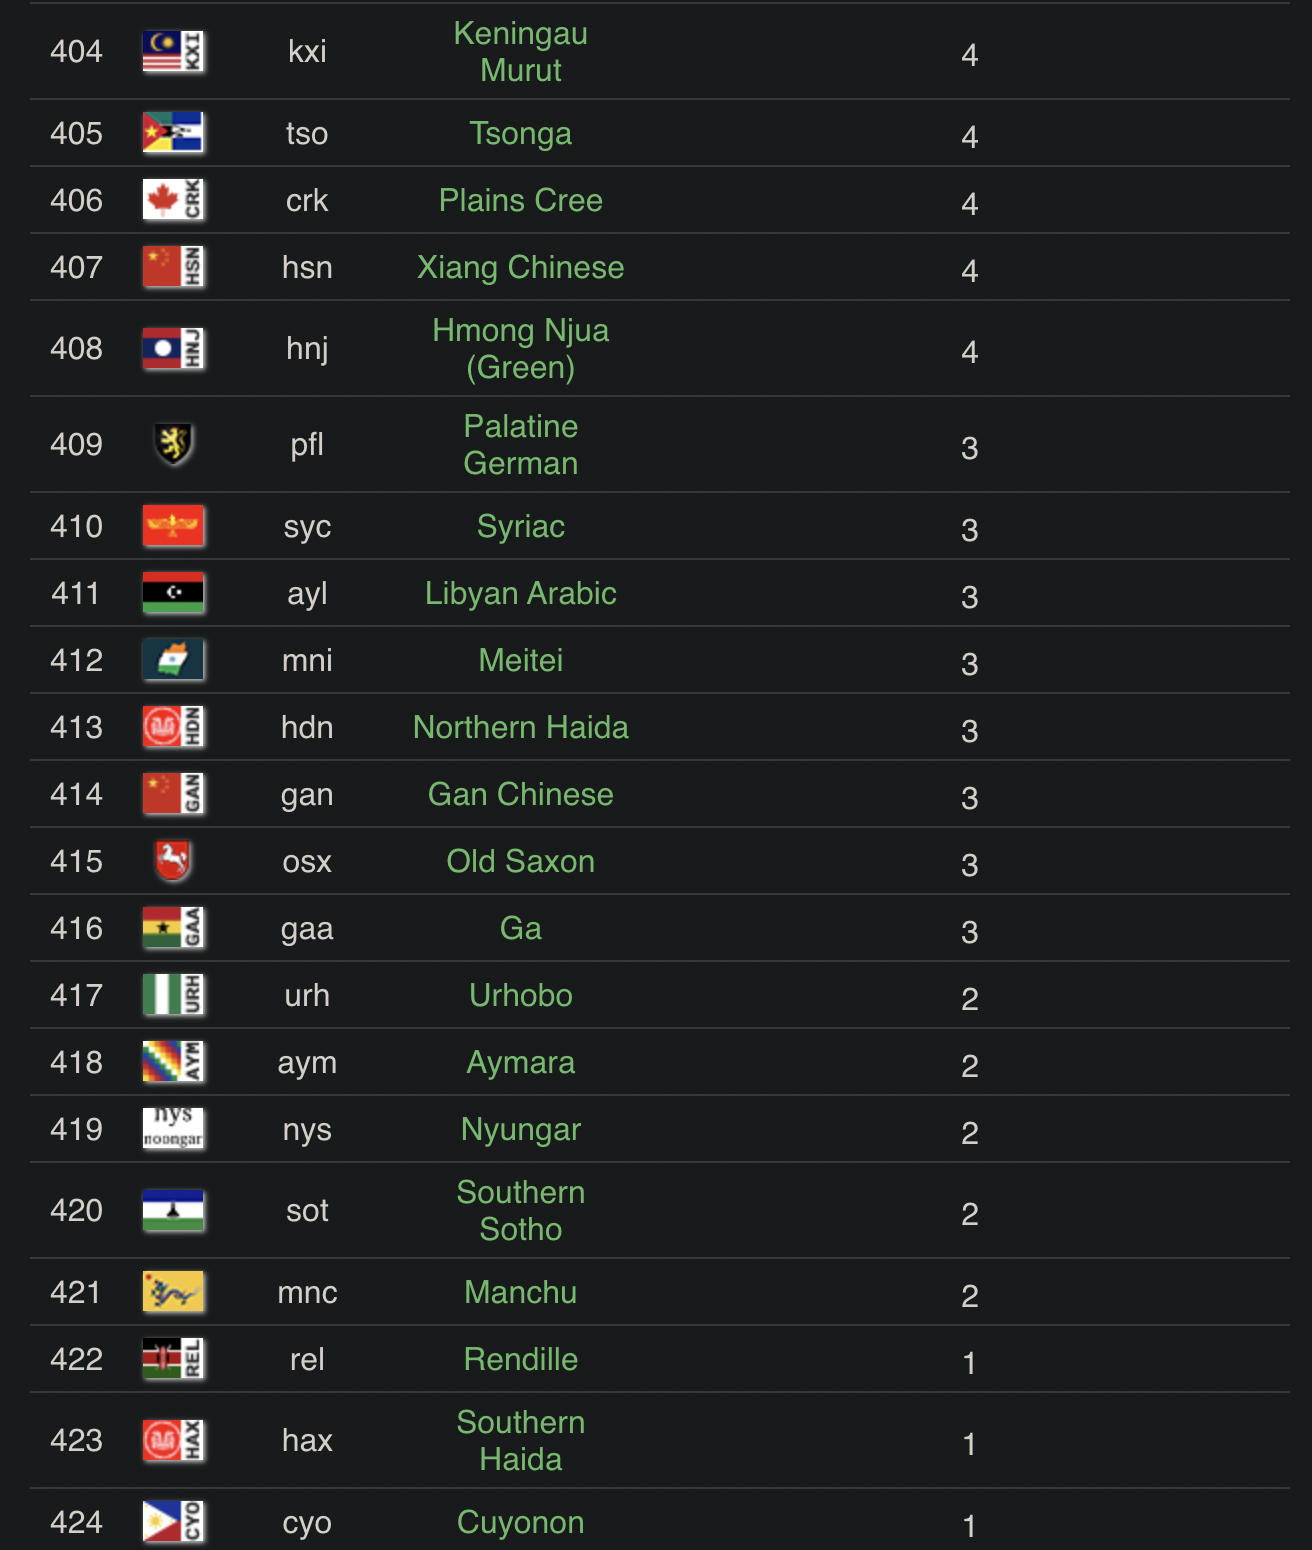
\includegraphics[width=0.46\linewidth]{images/tatoeba_bottom_20_lang.png}
    \caption{Tatoeba top 20 and bottom 20 languages based on sentences count \cite{tatoeba}}
    \label{fig:tatoeba_top_bottom_languages}
\end{figure}

Sentences typically consist of everyday phrases such as 'I have to go to sleep', 'That is intriguing', and 'Where do you live?' They may also include single-word exclamations like 'Speak!' or 'Look!' Additionally, multiple sentences such as 'You may write in any language you want. On Tatoeba, all languages are considered equal', and 'Guns don't kill people. People kill people' can be found inside the corpus. A few of them also include human names, 'Compare your answer with Tom's', 'Muiriel is 20 now'. All of the sentences are straightforward and literal, without the use of linguistic devices such as metaphors or sarcasm. Therefore, machine translation process should be straightforward on this level.

The languages chosen for evaluation in this study represent a wide overview, striking a balance between resources and diversity. Each language will then be translated into English (Many-to-English) and evaluated. The evaluation criteria encompass standard metrics such as BLEU (Bilingual Evaluation Understudy) \cite{papieni-2002-bleu}, METEOR (Metric for Evaluation of Translation with Explicit ORdering) \cite{lavie-2007-meteor} to capture nuances in translation quality. These metrics not only quantify the fidelity of translations but also offer insights into the models' adaptability and robustness across different linguistic pairs.

\begin{table}[htbp]
    \centering
    \begin{tabular}{|l|l|}
        \hline
        \textbf{No.} & \textbf{Language} \\
        \hline
        1            & Dutch             \\
        2            & Finnish           \\
        3            & French            \\
        4            & German            \\
        5            & Hebrew            \\
        6            & Hungarian         \\
        7            & Italian           \\
        8            & Japanese          \\
        9            & Mandarin Chinese  \\
        10           & Polish            \\
        11           & Portuguese        \\
        12           & Russian           \\
        13           & Spanish           \\
        14           & Turkish           \\
        15           & Ukrainian         \\
        \hline
    \end{tabular}
    \caption{List of chosen languages for evaluation}
\end{table}

Sentences dataset from Tatoeba is used \footnote{\url{https://tatoeba.org/}}. Languages that has more than fifty thousand sentences are selected. Accordingly, languages that are available for mbart is also selected based on the list here \footnote{\url{https://dl-translate.readthedocs.io/en/latest/available_languages/}}

For translation, all languages are translated into English as the target language. Then compare the true English sentence and the predicted one, calculated BLEU.

GPT-4 \cite{openai-2024-gpt4} try GPT and see

READ THIS \cite{intento-2020} (exactly what this paper should do, maybe compare results and find insights)

\section{Evaluation}

\section{Conclusion}

\printbibliography
\end{document}
